\documentclass[14pt]{extarticle}
\usepackage{amsmath}
\usepackage{amssymb}
%\usepackage{tikz}
%\usetikzlibrary{calc}
%\usetikzlibrary{trees}
\usepackage{hyperref}
\usepackage{graphicx}
\graphicspath{ {../../appdx/} }
\usepackage[top=0.75in, bottom=0.75in, left=0.75in, right=0.75in]{geometry}
%\newcommand*{\Scale}[2][4]{\scalebox{#1}{\ensuremath{#2}}}%
\usepackage[shortlabels]{enumitem}
\usepackage[most]{tcolorbox}
\definecolor{bg}{RGB}{255,249,227}
% \usepackage{showframe}
\title{\vspace{-5ex}Math 208 Appendix Review}
\date{\vspace{-10ex}}
%\usepackage{multicol}
%\setlength{\columnsep}{1cm}
\setlength{\parindent}{0pt}
\usepackage{parskip}
\setlength{\parskip}{10pt} % 1ex plus 0.5ex minus 0.2ex}
%\usepackage{ragged2e}

\begin{document}
	\maketitle	

\section{A.2: Operations on Polynomials}
\subsection{Multiplying}
Multiply
\begin{align*}
	(3x-5)(2x^2 +3x - 2) &= 3x(2x^2 +3x - 2) - 5(2x^2 +3x - 2) \\
	&= 3x^3 + 9x^2 - 6x -(10x^2 + 15x -10) \\
	&= 3x^3 + 9x^2 - 6x -10x^2 - 15x +10 \\
	&= 3x^3 - x^2 -21x+10
\end{align*}
Using vertical arrangement
\begin{align*}
	2x^2 &+ 3x - 2\\
	3x &-5\\
	\cline{1-2} 
	6x^3 &+ 9x^2 - 6x \\
	&- 10x^2 - 15x +10 \\
	\cline{1-2}
	6x^3 &- x^2 -21x +10
\end{align*}
\begin{tcolorbox}[enhanced jigsaw,colback=bg,boxrule=0pt,arc=0pt]
	\textbf{Important Products}
	\begin{align}
		(a-b)(a+b)&=a^2+b^2 \\
		(a+b)^2 &= a^2 +2ab + b^2 \\
		(a-b)^2 &= a^2 - 2ab +b^2
	\end{align}
\end{tcolorbox}
\subsection{Examples}
\begin{center}
	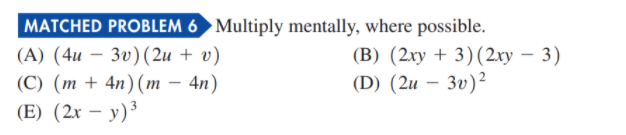
\includegraphics[width=0.9\linewidth]{a-2-1}
\end{center}

\section{A.3 Factoring Polynomials}
\subsection{Common Factors}
\begin{align*}
	4x^4y^2 - 8x^3y^3 + 12x^2y^2 & \\
	&= (4x^2y^2)x^2 -(4x^2y^2)2xy + (4x^2y^2)3 \\
	&= (4x^2y^2)(x^2 - 2xy+3)
\end{align*}

\subsection{Factor by Grouping}
\begin{align*}
	6x^2 + 11x +3 & \\
	&= 6x^2 + 2x + 9x + 3 \\
	&= (6x^2 + 2x) + (9x + 3) \\
	&= 2x(3x+1) + 3(3x+1) \\
	&= (2x+3)(3x+1)
\end{align*}

\begin{center}
	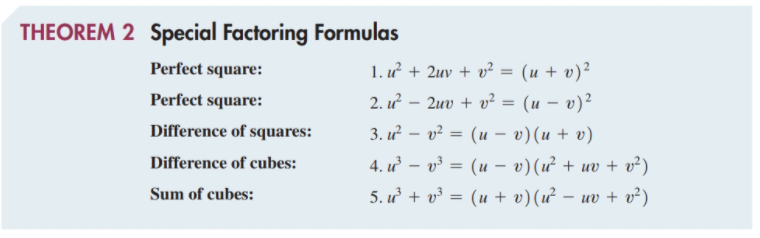
\includegraphics[width=1\linewidth]{a-3-1}
\end{center}

\subsection{Factor Completely}
\begin{align*}
	4x^2 - 12xy +9y^2 & \\
	&= (2x)^2 - 2(2x)(3y) + (3y)^2 \\
	&= (2x - 3y)^2
\end{align*}

\subsubsection{Examples}
\begin{center}
	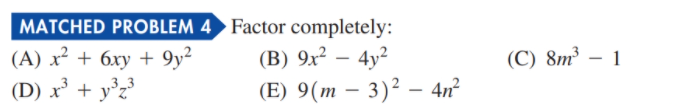
\includegraphics[width=0.9\linewidth]{a-3-2}
\end{center}

\section{A.4: Operations on Rational Expressions}
A Rational expression is a fraction where both the numerator and denominator are polynomials. Usually we denote this as $$R(x) = \frac{P(x)}{Q(x)}$$ where $Q(x)$ must not equal zero.

\subsection{Reduce to Lowest Terms}
\begin{align*}
	\frac{x^3-1}{x^2-1} & \\
	&= \frac{(x-1)(x^2 +x +1)}{(x-1)(x+1)} \\
	& = \frac{x^2 +x +1}{x+1}
\end{align*}

\section{A.5: Integer Exponents}
\begin{center}
	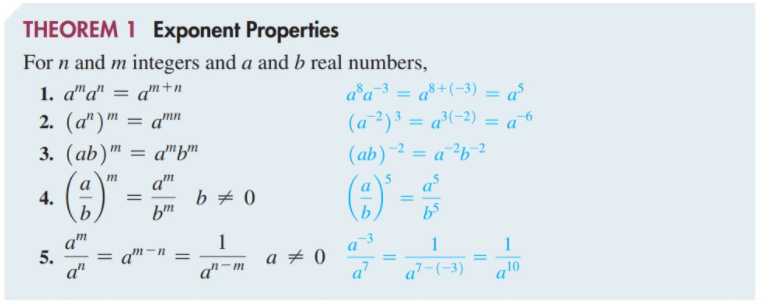
\includegraphics[width=1\linewidth]{a-5-1}
\end{center}
\begin{tcolorbox}[enhanced jigsaw,colback=bg,boxrule=0pt,arc=0pt]
	\textbf{Additional Properties}
	\begin{align*}
		a^0 &= 1 \\
		a^{-n} &= \frac{1}{a^n} 
	\end{align*}
\end{tcolorbox}
Simplify
\begin{align*}
	\left(\frac{y^{-5}}{y^{-2}}\right)^{-2} & \\
	&= \left(y^{-5}y^2\right)^{-2} \\
	&= \left(y^{-5+2}\right)^{-2} \\
	&= (y^{-3})^{-2} \\
	&= y^6
\end{align*}
Simplify
\begin{align*}
	\frac{1+x^{-1}}{1-x^{-2}} & \\
	&= \frac{1+ \frac{1}{x}}{1 - \frac{1}{x^2}} \\
	&= \left(\frac{x^2}{x^2}\right)\frac{1+ \frac{1}{x}}{1 - \frac{1}{x^2}} \\
	&= \frac{x^2 + x}{x^2 -1} \\
	&= \left(x\right)\frac{x+1}{(x+1)(x-1)} \\
	&= \frac{x}{x-1}
\end{align*}

\section{A.6: Rational Exponents and Radicals}
\subsection{nth Roots}
\begin{center}
	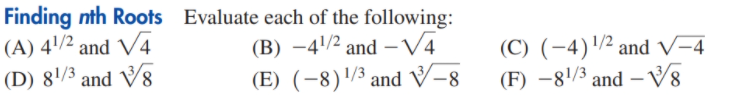
\includegraphics[width=1\linewidth]{a-6-1}
\end{center}
\subsection{Rational Exponents}
\begin{center}
	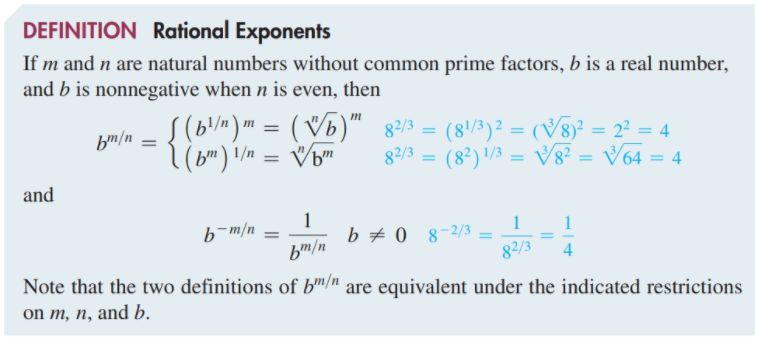
\includegraphics[width=1\linewidth]{a-6-2}
\end{center}
\begin{center}
	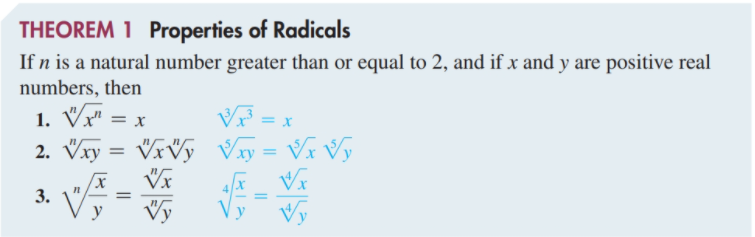
\includegraphics[width=1\linewidth]{a-6-3}
\end{center}

Often, in order to solve a problem we will need to rationalize either the numerator or the denominator. Here are two examples.
\begin{enumerate}
	\item Rationalize the Denominator
	\begin{align*}
		\frac{8x}{\sqrt{2x}} & \\
		&= \frac{8x}{\sqrt{2x}}\left(\frac{\sqrt{2x}}{\sqrt{2x}}\right) \\
		&= \frac{8x\sqrt{2x}}{2x} \\
		&= 4\sqrt{2x}
	\end{align*}
	\item Rationalize the Numerator
	\begin{align*}
		\frac{\sqrt{3+h}- \sqrt{3}}{h} & \\
		&= \frac{\sqrt{3+h}- \sqrt{3}}{h}\left(\frac{\sqrt{3+h}+ \sqrt{3}}{\sqrt{3+h}+ \sqrt{3}}\right) \\
		&= \frac{3+h- 3}{h(\sqrt{3+h}+ \sqrt{3})} \\
		&= \frac{h}{h(\sqrt{3+h}+ \sqrt{3})} \\
		&= \frac{1}{\sqrt{3+h}+ \sqrt{3}}
	\end{align*}
\end{enumerate}
\begin{center}
	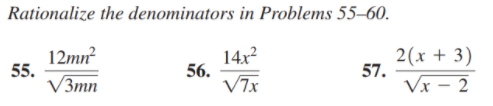
\includegraphics[width=.8\linewidth]{a-6-4}
	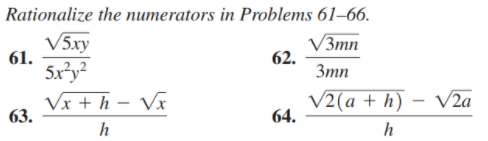
\includegraphics[width=.8\linewidth]{a-6-5}
\end{center}


\begin{align*}
\end{align*}

\begin{align*}
\end{align*}






\noindent\rule{\textwidth}{1pt}
{\footnotesize Copyright (C) 2021 Garold Dalton --- Released under GNU General Public License v3.0}


\cleardoublepage


\end{document}
